\input{preambuloSimple.tex}
\title{	
	\normalfont \normalsize 
	\textsc{{\bf Ingeniería de Servidores (2016-2017)} \\ Grado en Ingeniería Informática \\ Universidad de Granada} \\ [25pt] % Your university, school and/or department name(s)
	\horrule{0.5pt} \\[0.4cm] % Thin top horizontal rule
	\huge Instalación y configuración de servicios \\ % The assignment title
	\horrule{2pt} \\[0.5cm] % Thick bottom horizontal rule
}

\author{Manuel Jiménez Molina} % Nombre y apellidos

\date{\normalsize\today} % Incluye la fecha actual

%----------------------------------------------------------------------------------------
% DOCUMENTO
%----------------------------------------------------------------------------------------

\begin{document}
	
	\maketitle % Muestra el Título
	
	\newpage %inserta un salto de página
	
	\tableofcontents % para generar el índice de contenidos
	
	\listoffigures
	
	\listoftables
	
	\newpage
	
	%NOTA: en caso de problema al compilar, compruebe que tiene el paquete: texlive-babel-spanish.noarch  \\
	
	
	
	
	\newpage
	
	%----------------------------------------------------------------------------------------
	%	Cuestión 1
	%----------------------------------------------------------------------------------------
	
	\section{a) Liste los argumentos de yum necesarios para instalar,buscar y eliminar paquetes. b)¿Qué ha de hacer para que yum pueda tener acceso a Internet en el PC del aula?(Pistas: archivo de configuración en /etc,proxy: stargate.ugr.es:3128) c)¿Cómo añadimos un nuevo repositorio?}
	
	
	\subsection{a) Liste los argumentos de yum necesarios para instalar,buscar y eliminar paquetes.}
	
	Viendo el manual de yum\cite{ejercicio1-1} podemos ver los siguientes comandos:
	 
	\begin{itemize}
		
		\item Para instalar: yum install <paquete> 
			\begin{figure}[H] 
				\centering
				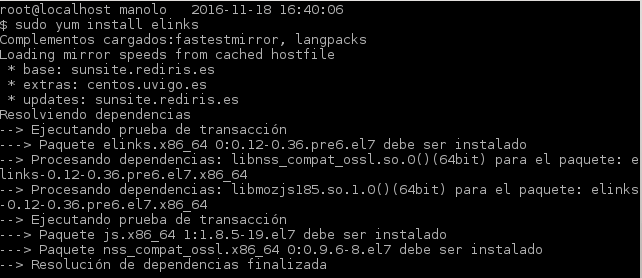
\includegraphics[scale=0.5]{ejercicio1-1-1.png} 
				\label{figura1} 
				\caption{Uso de yum install}
			\end{figure} 
			
		\item Para buscar: yum search <paquete>
			 \begin{figure}[H] 
			 	\centering
			 	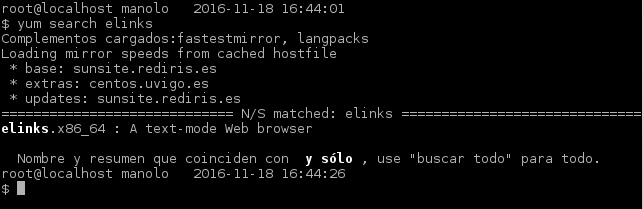
\includegraphics[scale=0.5]{ejercicio1-1-2.png} 
			 	\label{figura2} 
			 	\caption{Uso de yum search}
			 \end{figure}
			 
		\item Para eliminar: yum remove | erase <paquete>
			\begin{figure}[H] 
				\centering
				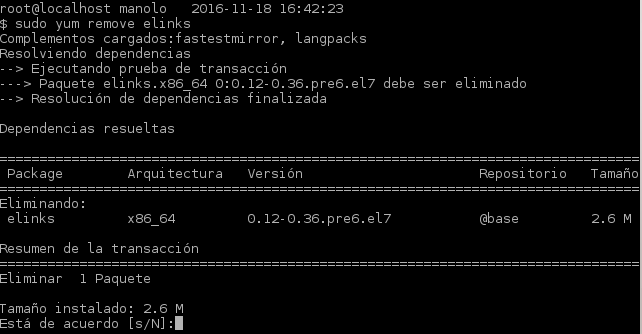
\includegraphics[scale=0.5]{ejercicio1-1-3.png} 
				\label{figura3} 
				\caption{Uso de yum remove}
			\end{figure} 
			
	\end{itemize}
	
	\subsection{b)¿Qué ha de hacer para que yum pueda tener acceso a Internet en el PC del aula?(Pistas: archivo de configuración en /etc,proxy: stargate.ugr.es:3128)}
	
	Tenemos que cambiar el proxy del archivo /etc/yum.conf\cite{ejercicio1-2}. Los pasos serían:
	
	\begin{itemize}
		\item Modificar el fichero /etc/yum.conf. Añadiremos la línea proxy=http://stargate.ugr.es:3128 :
			\begin{figure}[H] 
				\centering
				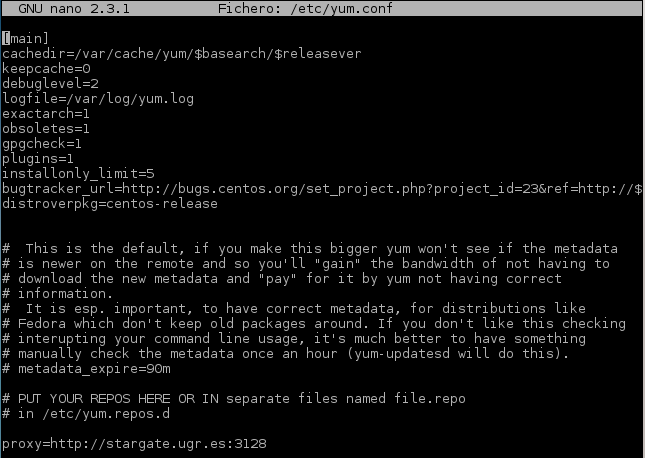
\includegraphics[scale=0.5]{ejercicio1-2-1.png} 
				\label{figura4} 
				\caption{Añadiendo el proxy en yum.conf}
			\end{figure}
		\item Comprobamos que como estoy con mi ordenador local en casa, yum no tendrá acceso a Internet debido a que el proxy indicado no sirve fuera de la red universitaria. Hacemos por ejemplo yum install y comprobamos que no funciona:
			\begin{figure}[H] 
				\centering
				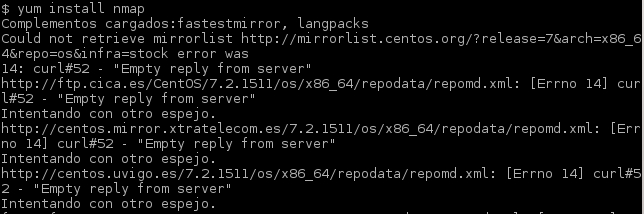
\includegraphics[scale=0.5]{ejercicio1-2-2.png} 
				\label{figura5} 
				\caption{Parte 1. Probando yum install con proxy cambiado}
			\end{figure}
			
			\begin{figure}[H] 
				\centering
				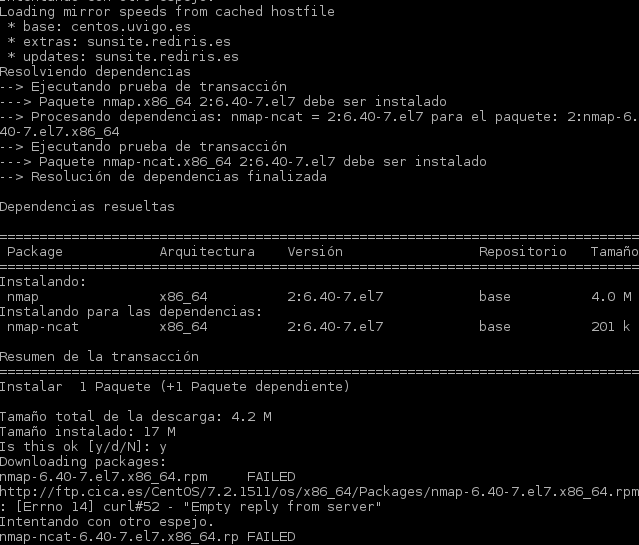
\includegraphics[scale=0.5]{ejercicio1-2-3.png} 
				\label{figura6} 
				\caption{Parte 2. Probando yum install con proxy cambiado}
			\end{figure}
			
			\begin{figure}[H] 
				\centering
				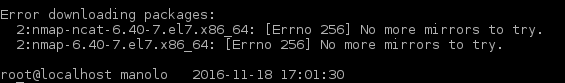
\includegraphics[scale=0.5]{ejercicio1-2-4.png} 
				\label{figura7} 
				\caption{Parte 3. Probando yum install con proxy cambiado}
			\end{figure}	
	\end{itemize}
	
	Podemos ver como finalmente no instala lo que le pedimos (nmap) ya que es incapaz de acceder Internet para detectar los paquetes necesarios. Puesto que desde casa esto funciona, suponemos que en los ordenadores de clase al no tener este proxy no les será posible acceder a Internet.
	
	\subsection{c)¿Cómo añadimos un nuevo repositorio?}

	Se pueden añadir repositorios de varios formas\cite{ejercicio1-3,ejercicio1-4,ejercicio1-5}:
	\begin{itemize}
		\item Mediante el comando yum-config-manager --add-repo repositoryURL:
		\begin{itemize}
			\item Añadimos nuevo repositorio con yum-config-manager:
				\begin{figure}[H] 
					\centering
					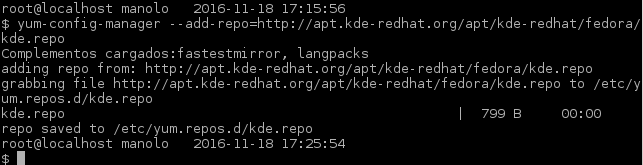
\includegraphics[scale=0.5]{ejercicio1-3-1.png} 
					\label{figura8} 
					\caption{Uso de yum-config-manager para añadir repositorio}
				\end{figure}
			\item Activamos el repositorio que acabamos de añadir.
				\begin{figure}[H] 
					\centering
					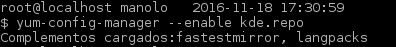
\includegraphics[scale=0.5]{ejercicio1-3-2.png} 
					\label{figura9} 
					\caption{Activación del repositorio con yum-config-manager}
				\end{figure}
			\item Comprobamos que se ha creado correctamente. Para ello el nuevo repositorio tendrá un archivo en /etc/yum.repos.d/:
				\begin{figure}[H] 
					\centering
					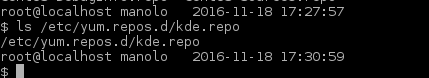
\includegraphics[scale=0.5]{ejercicio1-3-3.png} 
					\label{figura10} 
					\caption{Comprobar que un nuevo repositorio se creó en /etc/yum.repos.d/}
				\end{figure}
			\item Comprobar contenido del nuevo repositorio kde.repo:
				\begin{figure}[H] 
					\centering
					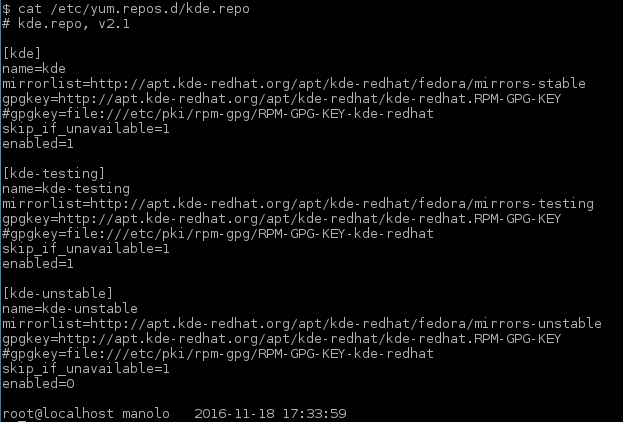
\includegraphics[scale=0.5]{ejercicio1-3-4.png} 
					\label{figura11} 
					\caption{Ver contenido de kde.repo}
				\end{figure}
			
		\end{itemize}
		 		
		\item Añadir los archivos de definición del repositorio en /etc/yum.repos.d/. Sería incluir el archivo kde.repo de forma manual, con la información que se ve en la figura anterior.	 
	\end{itemize}
	
	%----------------------------------------------------------------------------------------
	%	Cuestión 2
	%----------------------------------------------------------------------------------------
	
	\section{a) Liste los argumentos de apt necesarios para instalar, buscar y eliminar paquetes. b)¿Qué ha de hacer para que apt pueda tener acceso a Internet en el PC del aula?(Pistas: archivo de configuración en /etc, proxy:stargate.ugr.es:3128) c)¿Cómo añadimos un nuevo repositorio?}
	
	
	\subsection{a) Liste los argumentos de apt necesarios para instalar, buscar y eliminar paquetes.}
	
	Viendo el manual de Linux\cite{ejercicio2-1} podemos saber los argumentos de apt necesarios para:
	
	\begin{itemize}
		\item Para instalar: apt install <paquete>
			\begin{figure}[H] 
				\centering
				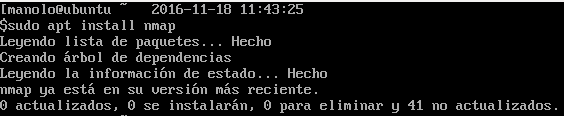
\includegraphics[scale=0.5]{ejercicio2-1-1.png} 
				\label{figura12} 
				
				\caption{Uso de apt install para gedit}
			\end{figure}
		 
		\item Para buscar: apt search <paquete>
			\begin{figure}[H] 
				\centering
				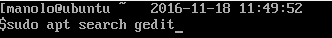
\includegraphics[scale=0.5]{ejercicio2-1-2.png} 
				\label{figura13} 
				
				\caption{Uso de apt search para gedit}
			\end{figure}
			\begin{figure}[H] 
				\centering
				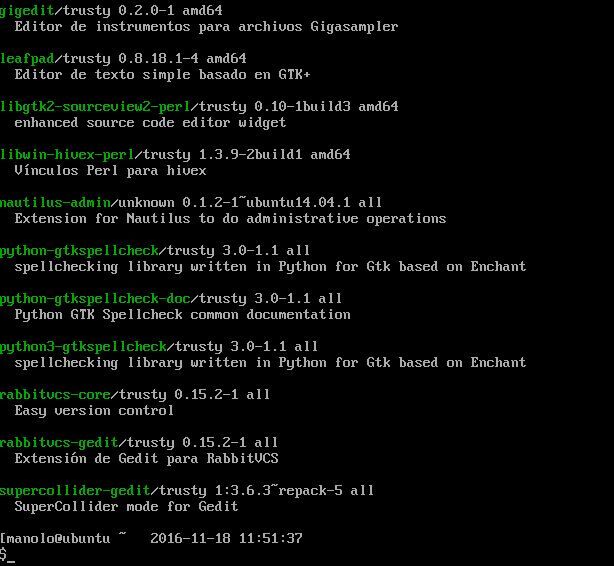
\includegraphics[scale=0.5]{ejercicio2-1-3.png} 
				\label{figura14} 
				
				\caption{Paquetes mostrados por apt search para gedit}
			\end{figure}
		\item Para eliminar: apt remove <paquete>  o apt-get purge <paquete>
			\begin{figure}[H] 
				\centering
				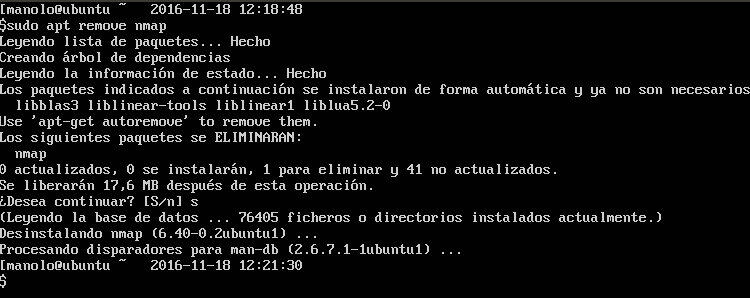
\includegraphics[scale=0.5]{ejercicio2-1-4.png} 
				\label{figura15} 
				
				\caption{Uso de apt remove para borrar el paquete nmap}
			\end{figure}
	\end{itemize}
	
	\subsection{b)¿Qué ha de hacer para que apt pueda tener acceso a Internet en el PC del aula?(Pistas: archivo de configuración en /etc, proxy:stargate.ugr.es:3128)}
	
	Siguiendo el manual de apt.conf\cite{ejercicio2-2} debemos de:
	\begin{itemize}
		\item Primero tenemos que crear un archivo llamado apt.conf en la ruta /etc/apt.
		\begin{figure}[H] 
			\centering
			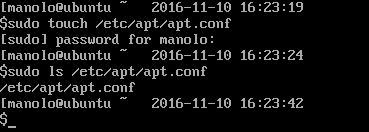
\includegraphics[scale=0.5]{ejercicio2-2-1.png} 
			\label{figura16} 
			
			\caption{Creación de archivo apt.conf}
		\end{figure}
		\item Añadimos dentro del archivo la linea Acquire::http::Proxy "http://stargate.ugr.es:3128"
		\begin{figure}[H] 
			\centering
			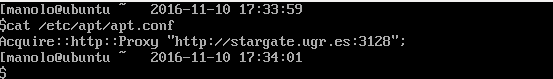
\includegraphics[scale=0.5]{ejercicio2-2-2.png} 
			\label{figura17} 
			
			\caption{Ver contenido apt.conf}
		\end{figure}
		\item Comprobamos que ahora no debería dejarnos instalar paquetes, ya que estoy en mi ordenador local. Hacemos apt update y comprobamos su funcionamiento.
			\begin{figure}[H] 
				\centering
				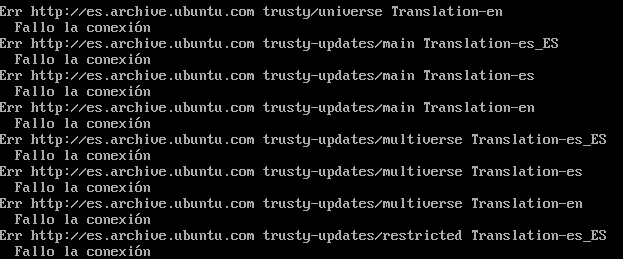
\includegraphics[scale=0.5]{ejercicio2-2-3.png} 
				\label{figura18} 
				
				\caption{Comprobación de no conexión con nuevo proxy}
			\end{figure}
	\end{itemize}
	
	Podemos ver como no permite conectarse al proxy indicado al cambiarlo. En cambio antes si dejaba ir. Como conclusión el añadir un proxy sirve para cambiar el comportamiento a la hora de buscar los paquetes de apt.
	
	\subsection{c)¿Cómo añadimos un nuevo repositorio?}
	
	Para añadir repositorios usamos la siguiente orden\cite{ejercicio2-3}: 
	\begin{itemize}
		\item Usar add-apt-repository <repositorio>
			\begin{figure}[H] 
				\centering
				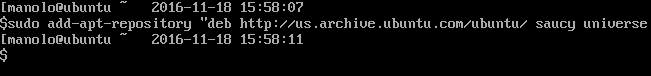
\includegraphics[scale=0.5]{ejercicio2-3-1.png} 
				\label{figura19} 
				
				\caption{Uso de add-apt-repository}
			\end{figure}
		\item Añadir en el archivo /etc/apt/sources.list el repositorio. La orden add-apt-repository hace justo esto, de modo que no tengas que buscar el archivo y añadirlo tú.
			\begin{figure}[H] 
				\centering
				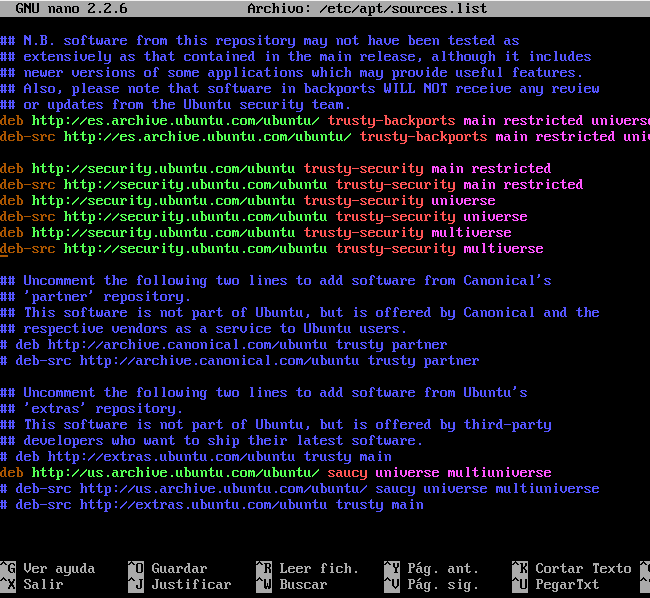
\includegraphics[scale=0.5]{ejercicio2-3-2.png} 
				\label{figura20} 
				
				\caption{Añadir nuevo repositorio modificando /etc/apt/sources.list}
			\end{figure}
		Abajo del archivo podemos ver el repositorio añadido "deb http://us.archive.ubuntu.com/ubuntu/ saucy universe multiverse"
	\end{itemize}
	
	
	%----------------------------------------------------------------------------------------
	%	Cuestión 3
	%----------------------------------------------------------------------------------------
	
	\section{a) ¿Con qué comando puede abrir/cerrar un puerto usando ufw? Muestre un ejemplo de cómo lo ha hecho b) ¿Con qué comando puede abrir/cerrar un puerto usando firewall-cmd en CentOS? Muestre un ejemplo de cómo lo ha hecho c) Utilice el comando nmap para ver que,efectivamente, los puertos están accesibles}
	
	

	\subsection{a) ¿Con qué comando puede abrir/cerrar un puerto usando ufw?}
	
	Revisando el manual de ufw\cite{ejercicio3-1} podemos ver sus diferentes órdenes, entre ellas se encuentran las necesarias para abrir y cerrar puertos.
	
	\begin{itemize}
		\item Abrir puertos con ufw allow <puerto>/protopocolo. Por ejemplo: ufw allow 80/tcp
		\item Cerrar puertos con ufw allow <puerto>/protopocolo. Por ejemplo: ufw deny 80/tcp 
	\end{itemize}
	
	Primero vamos a habilitar ufw y abrir el puerto 200 con protocolo tcp. Terminamos comprobando que está habilitado con "ufw status":
	
	\begin{figure}[H] 
		\centering
		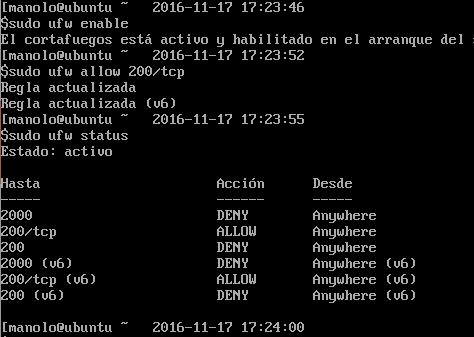
\includegraphics[scale=0.5]{ejercicio3-1-1.png} 
		\label{figura21} 
		
		\caption{Habilitar puerto 200/tcp con ufw}
	\end{figure}
	
	Finalmente cerramos ese puerto y comprobamos que se ha cerrado bien:
	
	\begin{figure}[H] 
		\centering
		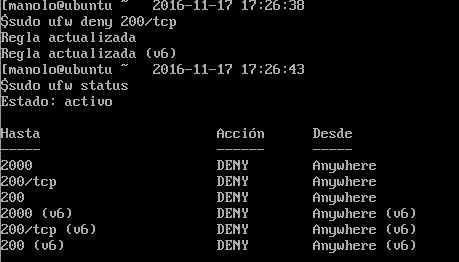
\includegraphics[scale=0.5]{ejercicio3-1-2.png} 
		\label{figura22} 
		
		\caption{Deshabilitar puerto 200/tcp con ufw}
	\end{figure}
	
	\subsection{b) ¿Con qué comando puede abrir/cerrar un puerto usando firewall-cmd en CentOS? Muestre un ejemplo de cómo lo ha hecho}
	
	Consultando el manual de firewall-cmd averiguamos los comandos necesarios para abrir/cerrar puertos\cite{ejercicio3-2,ejercicio3-3}:
	
	\begin{itemize}
		\item Abrir puertos. Se pueden realizar de varios modos si queremos que los cambios permanezcan aunque se reinicie el sistema.
		\begin{itemize}
			\item Abrir puerto para que siga estando hasta que se reinicie el sistema. Se usa el comando \textbf{firewall-cmd --add-port=443/tcp}.
			 
			 \begin{figure}[H] 
			 	\centering
			 	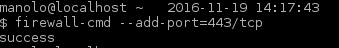
\includegraphics[scale=1]{ejercicio3-2-1.png} 
			 	\label{figura23} 
			 	
			 	\caption{Abrir puerto no permanente con firewall-cmd}
			 \end{figure}
			 
			 Comprobamos que el puerto ha sido abierto correctamente, para ello usamos el comando \textbf{firewall-cmd --list-ports}.
			 
			 \begin{figure}[H] 
			 	\centering
			 	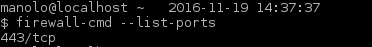
\includegraphics[scale=1]{ejercicio3-2-2.png} 
			 	\label{figura24} 
			 	
			 	\caption{Comprobar puerto no permanente con firewall-cmd}
			 \end{figure}
			

			
			\item Abrir puerto para que siga siendo permanente independientemente de los reinicios del sistema. Se usa el comando \textbf{firewall-cmd --permanent --add-port=443/tcp}.
			\begin{figure}[H] 
				\centering
				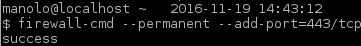
\includegraphics[scale=1]{ejercicio3-2-3.png} 
				\label{figura25} 
				
				\caption{Abrir puerto permanente con firewall-cmd}
			\end{figure}
			
			Comprobamos que el puerto ha sido abierto correctamente, para ello usamos el comando \textbf{firewall-cmd --permanent --list-ports}.
			
			\begin{figure}[H] 
				\centering
				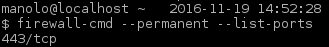
\includegraphics[scale=1]{ejercicio3-2-4.png} 
				\label{figura26} 
				
				\caption{Comprobar puerto permanente con firewall-cmd}
			\end{figure}
			
			
		\end{itemize}
		\item Cerrar puertos. Se cerrarán y comprobarán con distintos comandos si son permanentes tras el reinicio o no.
			\begin{itemize}
				\item Cerrar puertos no permanente con el comando \textbf{firewall-cmd --remove-port=443/tcp} y su comprobación con el comando \textbf{firewall-cmd --list-ports}.
				\begin{figure}[H] 
					\centering
					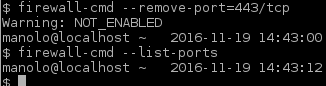
\includegraphics[scale=0.7]{ejercicio3-2-5.png} 
					\label{figura27} 
					
					\caption{Cerrado y comprobación puerto no permanente con firewall-cmd}
				\end{figure}
				
				Podemos ver como el puerto ya no se muestra. Ha sido cerrado correctamente.
				
				\item Cerrar puertos permanentes con el comando \textbf{firewall-cmd --permanent --remove-port=443/tcp} y su comprobación con el comando \textbf{firewall-cmd --permanent --list-ports}.
				\begin{figure}[H] 
					\centering
					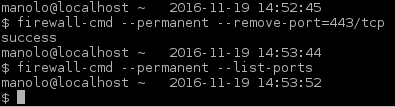
\includegraphics[scale=0.7]{ejercicio3-2-6.png} 
					\label{figura28} 
					
					\caption{Cerrado y comprobación puerto permanente con firewall-cmd}
				\end{figure}
			\end{itemize}
	\end{itemize}
	
	\subsection{c) Utilice el comando nmap para ver que,efectivamente, los puertos están accesibles}

	Vamos a abrir/cerrar el puerto 22 de ssh en Ubuntu Server que tiene un servicio asociado (demonio sshd) con ufw y comprobamos como se ve ese puerto según las diferentes combinaciones en el interior y exterior (otra máquina, por ejemplo la anfitriona)usando para ello nmap\cite{ejercicio3-4}:
	
	
	\begin{itemize}
		\item Escenario 1: puerto 22 cerrado (deny) con ufw y servicio de ssh parado.
			\begin{itemize}
				\item a) desde localhost: cerrado.
					\begin{figure}[H] 
						\centering
						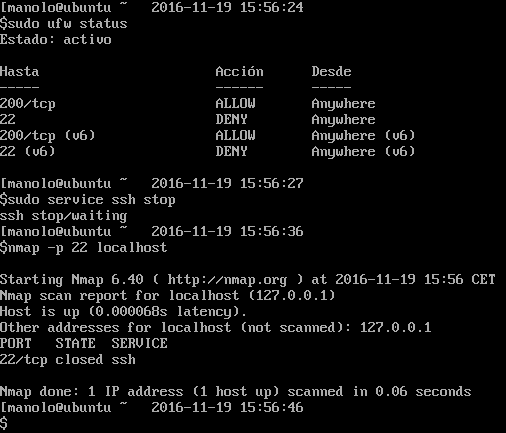
\includegraphics[scale=0.6]{ejercicio3-3-1.png} 
						\label{figura29} 
						
						\caption{Escenario 1, localhost usando nmap}
					\end{figure}
				\item b) desde fuera: filtrado.
					\begin{figure}[H] 
						\centering
						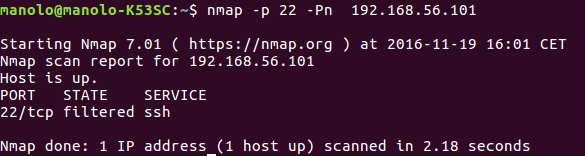
\includegraphics[scale=0.6]{ejercicio3-3-2.png} 
						\label{figura30} 
						
						\caption{Escenario 1, desde fuera usando nmap}
					\end{figure}
			\end{itemize}
		\item Escenario 2: puerto 22 abierto. (allow) con ufw y servicio de shh parado.
			\begin{itemize}
				\item a) desde localhost: cerrado.
					\begin{figure}[H] 
						\centering
						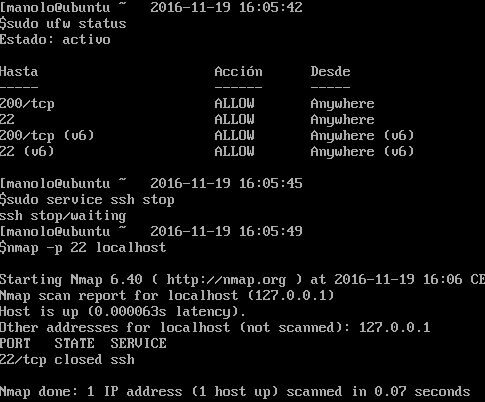
\includegraphics[scale=0.6]{ejercicio3-3-3.png} 
						\label{figura31} 
						
						\caption{Escenario 2, localhost usando nmap}
					\end{figure}
				\item b) desde fuera: cerrado.
					\begin{figure}[H] 
						\centering
						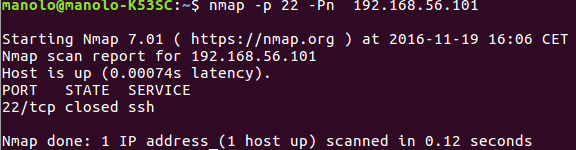
\includegraphics[scale=0.6]{ejercicio3-3-4.png} 
						\label{figura32} 
						
						\caption{Escenario 2, desde fuera usando nmap}
					\end{figure}
			\end{itemize}
		\item Escenario 3: puerto cerrado (deny) con ufw y servicio de ssh escuchando.
			\begin{itemize}
				\item a) desde localhost: open.
					\begin{figure}[H] 
						\centering
						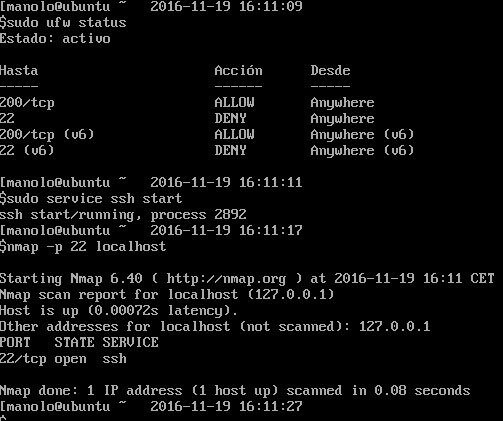
\includegraphics[scale=0.6]{ejercicio3-3-5.png} 
						\label{figura33} 
						
						\caption{Escenario 3, localhost usando nmap}
					\end{figure}
				\item b) desde fuera: filtrado.
					\begin{figure}[H] 
						\centering
						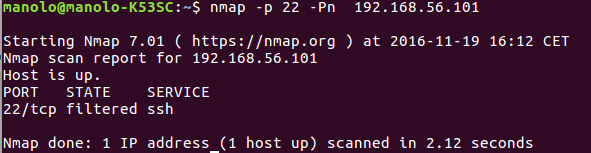
\includegraphics[scale=0.6]{ejercicio3-3-6.png} 
						\label{figura34} 
						
						\caption{Escenario 3, desde fuera usando nmap}
					\end{figure}
			\end{itemize}
		\item Escenario 4: puerto 22 abierto con ufw y servicio de ssh escuchando.
			\begin{itemize}
				\item a) desde localhost: open.
					\begin{figure}[H] 
						\centering
						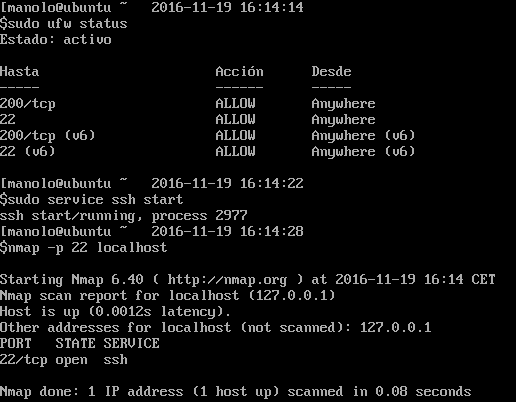
\includegraphics[scale=0.6]{ejercicio3-3-7.png} 
						\label{figura35} 
						
						\caption{Escenario 4, localhost usando nmap}
					\end{figure}
				\item b) desde fuera: open.
					\begin{figure}[H] 
						\centering
						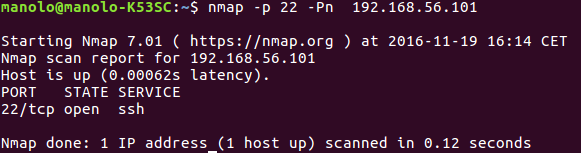
\includegraphics[scale=0.6]{ejercicio3-3-8.png} 
						\label{figura36} 
						
						\caption{Escenario 4, desde fuera usando nmap}
					\end{figure}
			\end{itemize}
	\end{itemize}
	
	
	Tras comprobar estos cuatro estados llegamos a las siguientes conclusiones:
	\begin{itemize}
		\item Si te quieres conectar desde fuera, la máquina a la que te conectas tiene que tener su puerto permitido por el firewall y además que un proceso esté escuchando en dicho puerto.
		\item Si te conectas desde dentro, podrás hacerlo siempre que tengas un proceso escuchando en el puerto deseado. No importa si el puerto en el firewall está abierto o cerrado ya que este solo controla las conexiones entrantes. 
	\end{itemize}
	
	%	Cuestión 4
	%-----------------------------------------------
	\section{¿Qué diferencia hay entre telnet y ssh?}
	
	Telnet\cite{ejercicio4-1,ejercicio4-4}: Protocolo para conexiones remotas por TCP. No es segura, ya que la información no es cifrada (la envía en texto plano) y terceros pueden obtenerla del tráfico que se transmite. Usa el puerto 23. Para conocer más a fondo este protocolo, podemos ver su RFC\cite{ejercicio4-2,ejercicio4-3}.
	\\
	
	SSH\cite{ejercicio4-5,ejercicio4-6}: Protocolo de red que permite transmitir información sobre un canal seguro. Los datos que pasan por el canal va cifrados por lo que se mantiene su seguridad. Proporciona aplicaciones gráficas sobre una red (X11). Comúnmente es usado en lugar de Telnet. Usa el puerto 22. Para conocer más a fondo este protocolo, podemos ver su RFC\cite{ejercicio4-7}.
	\\
	
	Como conclusión, las diferencias son:
	\begin{itemize}
		\item ssh es más seguro que Telnet, ya que Telnet envía información en texto plano y ssh cifrada. 
		\item ssh es más usado que Telnet, debido a su seguridad.
		\item ssh proporciona interacción de forma gráfica en la red (X11), Telnet no.
		\item ssh añade más sobrecarga de banda ancha que Telnet, debido a que su información es cifrada y necesita mayor tamaño.
		\item Telnet usa el puerto 23 y ssh el 22.
	\end{itemize} 
	
	
	%----------------------------------------------------------------------------------------
	%	Cuestión 5
	%----------------------------------------------------------------------------------------
	
	\section{a) ¿Para qué sirve la opción -X? b) Ejecute remotamente, es decir, desde la máquina anfitriona (si tiene Linux) o desde la otra máquina virtual, el comando gedit en una sesión abierta con ssh. ¿Qué ocurre?}
	
	
	\subsection{a) ¿Para qué sirve la opción -X?}
	
	La opción -X sirve para \cite{ejercicio5-1,ejercicio5-2,ejercicio5-3} habilitar X11. X11 es un servicio de ventanas que permite interacción de forma gráfica en red. Esto quiere decir que si usamos ssh podemos ejecutar programas que están en una máquina remota sin tener que instalar el programa en local y X11 es quien se encarga de enseñarnos dicha ejecución, ya que proporciona una ventana donde podremos ver dicha ejecución.
	
	
	\subsection{b) Ejecute remotamente, es decir, desde la máquina anfitriona (si tiene Linux) o desde la otra máquina virtual, el comando gedit en una sesión abierta con ssh. ¿Qué ocurre?}
	
	Antes de empezar a ejecutar remotamente, tenemos aseguraremos que Ubuntu Server y nuestra máquina anfitriona Ubuntu Desktop se puedan comunicar correctamente por ssh. Para ello en VirtualBox configuramos la red de la máquina virtualizada de Ubuntu Server del siguiente modo:
	
	\begin{itemize}
		\item Se establece un adaptador en modo NAT.
		\begin{figure}[H] 
			\centering
			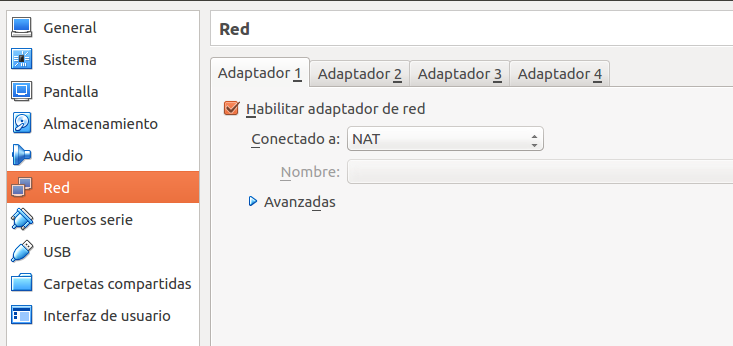
\includegraphics[scale=0.5]{ejercicio5-2-1.png} 
			\label{figura37} 
			
			\caption{Configuración de red para máquina virtual, adaptador 1}
		\end{figure}
		\item Se crea un segundo adaptador como adaptador-solo-anfitrión.
		\begin{figure}[H] 
			\centering
			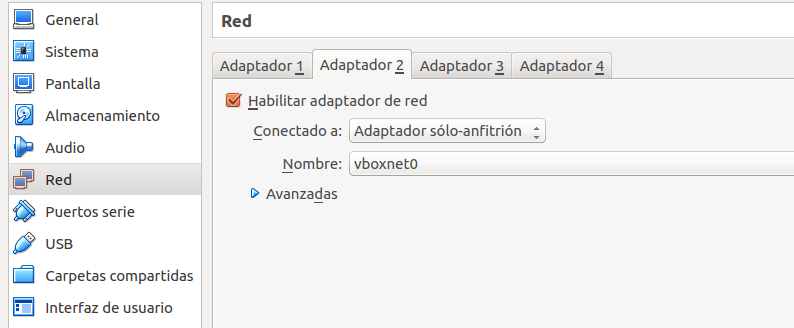
\includegraphics[scale=0.5]{ejercicio5-2-2.png} 
			\label{figura38} 
			
			\caption{Configuración de red para máquina virtual, adaptador 2}
		\end{figure}
	\end{itemize}
	
	Después preparamos el ssh, instalando el openssh-server, para obtener archivos del demonio ssh\cite{ejercicio5-4}:
	
	\begin{itemize}
		\item sudo apt-get install openssh-server
	\end{itemize}  
	
	Leyendo más documentación sobre ssh, encontramos como ejecutar remotamente desde otra máquina virtual\cite{ejercicio5-5,ejercicio5-6}. Iremos paso por paso:
	
	\begin{itemize}
		\item Nos vamos al archivo de configuración de ssh /etc/ssh/ssh\_config para habilitar X11. Para ello se establece "ForwardX11 yes".	
			\begin{figure}[H] 
				\centering
				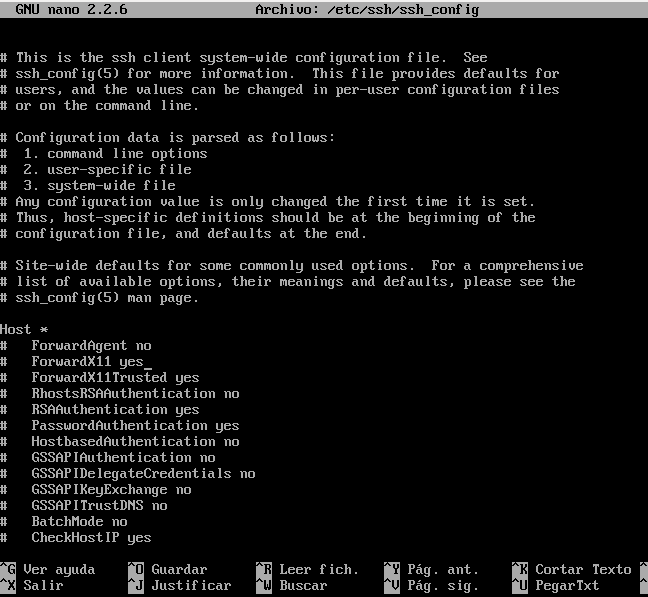
\includegraphics[scale=0.5]{ejercicio5-2-3.png} 
				\label{figura39} 	
				\caption{Habilitar X11 de ssh en fichero ssh\_config para permitir gráficos remotos}
			\end{figure}	
		\item Habilitamos X11 también en el archivo /etc/ssh/sshd\_config estableciendo "X11Forwarding yes":
			\begin{figure}[H] 
				\centering
				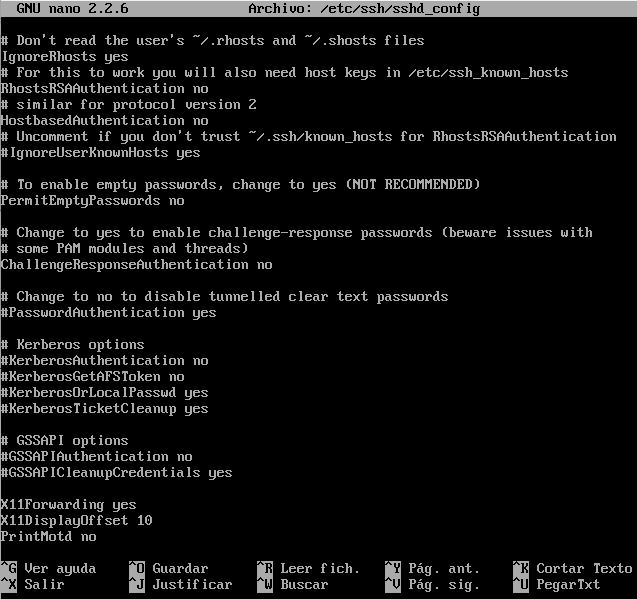
\includegraphics[scale=0.5]{ejercicio5-2-4.png} 
				\label{figura40} 	
				\caption{Habilitar X11 de ssh en fichero sshd\_config para permitir gráficos remotos}
			\end{figure}
		\item Reiniciamos el servicio ssh para que los cambios realizados se tengan en cuenta:
			\begin{itemize}
				\item sudo servicie ssh restart
				\begin{figure}[H] 
					\centering
					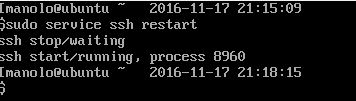
\includegraphics[scale=0.5]{ejercicio5-2-5.png} 
					\label{figura41} 
					\caption{Habilitar X11 de ssh en fichero sshd\_config para permitir gráficos remotos}
				\end{figure}
			\end{itemize}
		\item Usamos comando ifconfig\cite{ejercicio5-7} para comprobar las redes que tenemos.
			\begin{figure}[H] 
				\centering
				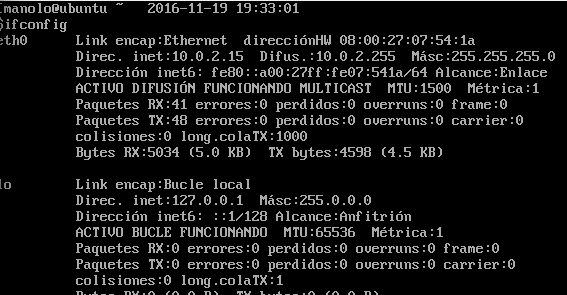
\includegraphics[scale=0.5]{ejercicio5-2-6.png} 
				\label{figura42} 
				\caption{Redes de la máquina Ubuntu Server}
			\end{figure}
		\item Vemos que no tenemos la interfaz eth1, debemos activarla.
			\begin{figure}[H] 
				\centering
				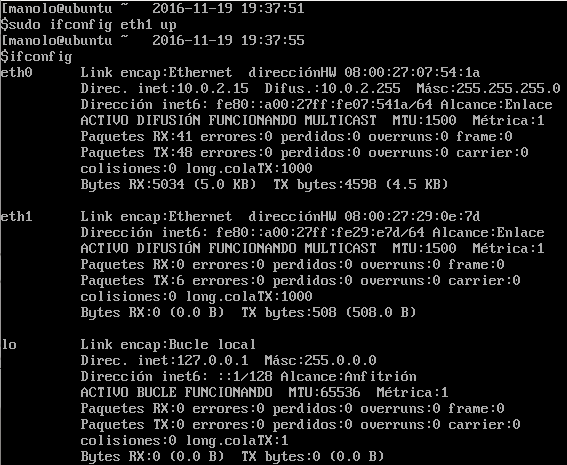
\includegraphics[scale=0.5]{ejercicio5-2-7.png} 
				\label{figura43} 
				\caption{Activar interfaz eth1}
			\end{figure}
		\item eth1 aún no tiene una dirección asociada. Configuramos la interfaz eth1 con el uso de dhclient\cite{ejercicio5-8}.
			\begin{figure}[H] 
				\centering
				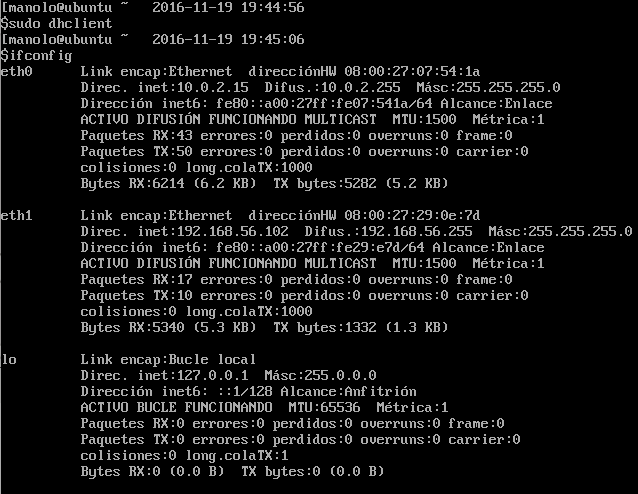
\includegraphics[scale=0.5]{ejercicio5-2-8.png} 
				\label{figura44} 
				\caption{Configurar interfaz eth1 con dhclient}
			\end{figure}
		\item Configuramos la interfaz\cite{ejercicio5-9} para que se quede de forma permanente cada vez que se reinicie en el sistema. Para ello vamos al archivo /etc/network/interfaces y añadimos la configuración de eth1 (será la misma que la de eth0).
			\begin{figure}[H] 
				\centering
				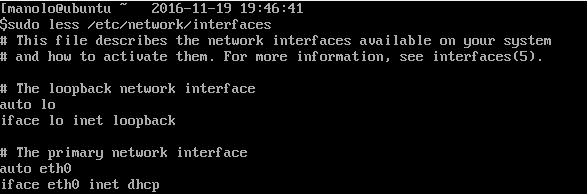
\includegraphics[scale=0.5]{ejercicio5-2-9.png} 
				\label{figura45} 
				\caption{Ver contenido de /etc/network/interfaces}
			\end{figure}
			\begin{figure}[H] 
				\centering
				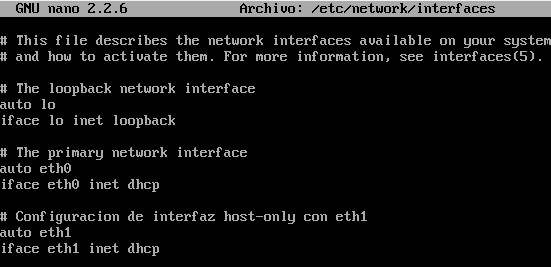
\includegraphics[scale=0.5]{ejercicio5-2-10.png} 
				\label{figura46} 
				\caption{Añadir configuración para interfaz eth1 en /etc/network/interfaces}
			\end{figure}
		\item Realizamos una copia del archivo "interfaces" modificado y lo llamaremos "interfaces.vap". De este modo podemos recurrir a él en caso de pérdida del original.
			\begin{figure}[H] 
				\centering
				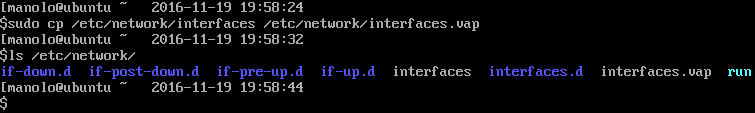
\includegraphics[scale=0.5]{ejercicio5-2-11.png} 
				\label{figura47} 
				\caption{Copia del archivo interfaces}
			\end{figure}
		\item Reiniciamos la máquina "sudo reboot" y comprobamos que las interfaces siguen estando usando ifconfig.
			\begin{figure}[H] 
				\centering
				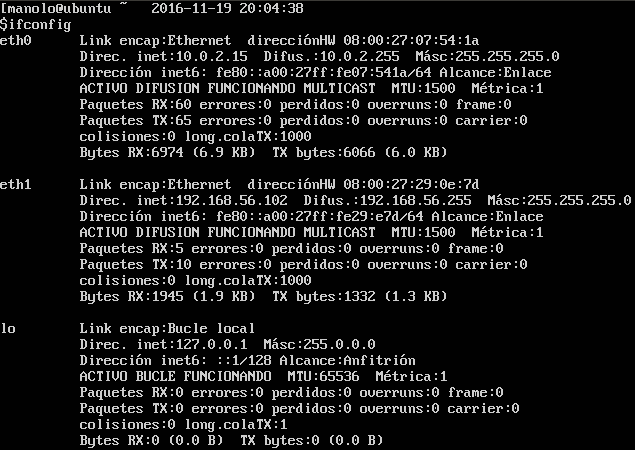
\includegraphics[scale=0.5]{ejercicio5-2-12.png} 
				\label{figura48} 
				\caption{Comprobación de interfaces tras los cambios}
			\end{figure}
		\item Comprobamos que el puerto ssh 22 está abierto por el firewall (ufw allow) y que el servicio ssh está escuchando.
			\begin{figure}[H] 
				\centering
				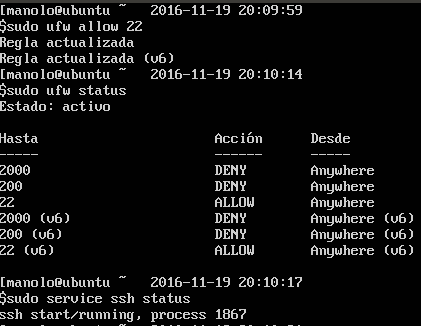
\includegraphics[scale=0.5]{ejercicio5-2-13.png} 
				\label{figura49} 
				\caption{Comprobación de firewall y servicio ssh}
			\end{figure}
		\item Finalmente, ya podemos conectarnos remotamente desde otra máquina. Vamos a comprobar que:
			\begin{itemize}
				\item Sin la opción -X de ssh no deja ejecutar gedit.
					\begin{figure}[H] 
						\centering
						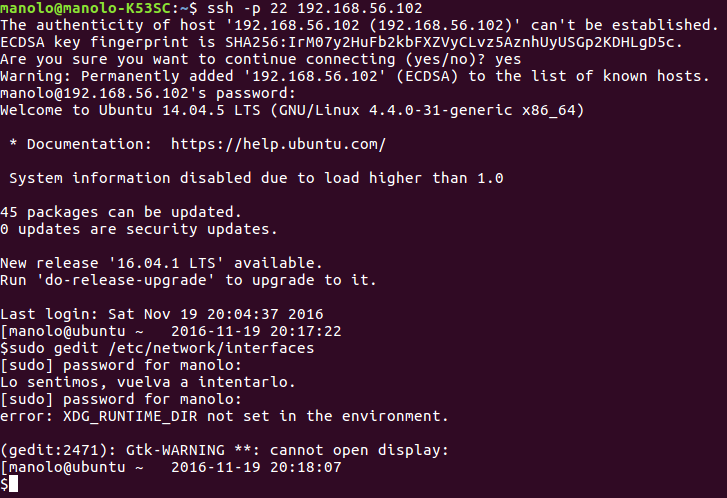
\includegraphics[scale=0.4]{ejercicio5-2-14.png} 
						\label{figura50} 
						\caption{Uso remoto de ssh sin opción -X}
					\end{figure}
				\item Con la opción -X de ssh permite ejecutar gedit.
					\begin{figure}[H] 
						\centering
						\includegraphics[scale=0.5]{ejercicio5-2-15.png} 
						\label{figura51} 
						\caption{Uso remoto de ssh con opción -X}
					\end{figure}
			\end{itemize}
	\end{itemize}
	
	
	%----------------------------------------------------------------------------------------
	%	Cuestión 6
	%----------------------------------------------------------------------------------------
	
	\section{Muestre la secuencia de comandos y las modificaciones a los archivos correspondientes para permitir acceder a la consola remota sin introducir la contraseña. Pruebe que funciona. (Pistas: ssh-keygen, ssh-copy-id)}
	
	Con las pistas que nos dan, sabemos que ssh-keygen\cite{ejercicio6-1} se usa para generación, gestión y conversión de claves de autenticación (clave pública y privada). Por otra parte ssh-copy-id\cite{ejercicio6-2} se usa para instalar una clave pública en una máquina remota autorizada.
	\\
	
	Indagando un poco más, encontramos en RedHat documentación de sobre "gestión remota con SSH" que hace uso de las órdenes descritas antes. Las desventajas de introducir la contraseña cada vez que nos conectamos remotamente con ssh son las siguientes: 
	\begin{itemize}
		\item El proceso inicial de configuración de la conexión podría ser lento.
		\item ssh no escala bien con un mayor número de máquinas remotas.
		\item No hay una forma estándar de anular la clave de usuario en todos los hosts o invitados.
	\end{itemize}
	
	Por las desventajas comentadas, no tener que introducir la contraseña en cada conexión ssh remota es bueno. RedHat explica un proceso para acceder de forma remota con ssh sin tener introducir la contraseña (como se ha visto en las imágenes del ejercicio 5). Para ello realiza los siguientes pasos:
	
	\begin{itemize}
		\item Generación del par de claves ssh. Uso de ssh-keygen. Usaremos encriptación rsa y un tamaño de bits para ella de 2048.
			\begin{figure}[H] 
				\centering
				\includegraphics[scale=0.5]{ejercicio6-1.png} 
				\label{figura52} 
				\caption{Generación de claves con ssh-keygen}
			\end{figure}
		\item Vamos a ver los permisos de las claves.
			\begin{figure}[H]	
				\centering
				\includegraphics[scale=0.5]{ejercicio6-2.png} 
				\label{figura53} 
				\caption{Ver permisos de las claves generadas}
			\end{figure}
		\item Copiamos las claves a una máquina remota. Para ello usa ssh-copy-id.
			\begin{figure}[H]	
				\centering
				\includegraphics[scale=0.5]{ejercicio6-3.png} 
				\label{figura54} 
				\caption{Copiar clave pública a una máquina remota}
			\end{figure}
		\item Ahora ya podemos conectarnos por ssh sin que nos pida la contraseña.
			\begin{figure}[H]	
				\centering
				\includegraphics[scale=0.5]{ejercicio6-4.png} 
				\label{figura55} 
				\caption{Conexión remota por ssh sin introducir contraseña}
			\end{figure}
	\end{itemize}
	
	
	NOTA: La secuencia de comandos realizada en este ejercicio está realizada realmente para el usuario root, ya que en cada comando realizamos "sudo". Esto quiere decir que la sesión ssh que se inicia para "root" y no para el usuario "manolo".
	%----------------------------------------------------------------------------------------
	%	Cuestión 7
	%----------------------------------------------------------------------------------------
	\section{¿Qué archivo es el que contiene la configuración del servicio ssh? ¿Qué parámetro hay que modificar para evitar que el usuario root acceda? Cambie el puerto por defecto y compruebe que puede acceder.}
	
	El archivo que contiene la configuración del servicio ssh es /etc/ssh/sshd\_config\cite{ejercicio7-1}.
	\\
	
	El parámetro para evitar que el usuario root acceda\cite{ejercicio7-2} es:
	\begin{itemize}
		\item PermitRootLogin no
	\end{itemize}
	
	Antes que nada, he usado el comando sudo passwd root para establecer una contraseña al usuario root (antes no tenía ninguna).
	\\
	
	Ahora, vamos a comprobar que no deja acceder como root al poner el parámetro PermitRootLogin a no:
		\begin{itemize}
		\item Modificando archivo sshd\_config:
			\begin{figure}[H]	
				\centering
				\includegraphics[scale=0.5]{ejercicio7-1.png} 
				\label{figura56} 
				\caption{Modificando parámetro PermitRootLogin a no en ssh}
			\end{figure}
		\item Reiniciamos el servicio ssh:
			\begin{itemize}
				\item sudo service ssh restart
			\end{itemize}		
		\item Intentamos acceder como root remotamente y vemos como no nos deja iniciar sesión con root.
			\begin{figure}[H]	
				\centering
				\includegraphics[scale=0.5]{ejercicio7-2.png} 
				\label{figura57} 
				\caption{Conexion remota por ssh accediendo como root con PermitRootLogin no}
			\end{figure}
		\end{itemize}
	
	Para comprobar que realmente termina de funcionar, ponemos PermitRootLogin yes para que ahora sí nos deje acceder como root.
	\begin{itemize}
		\item Modificamos PermitRootLogin yes. 
			\begin{figure}[H]	
				\centering
				\includegraphics[scale=0.5]{ejercicio7-3.png} 
				\label{figura58} 
				\caption{Modificando parámetro PermitRootLogin a yes en ssh}
			\end{figure}
		\item Reiniciamos el servicio ssh:
		\begin{itemize}
			\item sudo service ssh restart
		\end{itemize}	 
		\item Comprobamos que deja acceder remotamente como root.
			\begin{figure}[H]	
				\centering
				\includegraphics[scale=0.5]{ejercicio7-4.png} 
				\label{figura59} 
				\caption{Conexion remota por ssh accediendo como root con PermitRootLogin yes}
			\end{figure}
	\end{itemize}
	
	
	El parámetro que hay que cambiar para modificar el puerto\cite{ejercicio7-3} por defecto del servicio ssh es:
	\begin{itemize}
		\item Port <numero>
	\end{itemize}
	
	Vamos a cambiar el puerto por defecto para ssh y vamos a comprobar que podemos acceder por ssh.
	\begin{itemize}
		\item Cambiamos el archivo sshd\_config y cambiamos por ejemplo el puerto a 1000.
			\begin{figure}[H]	
				\centering
				\includegraphics[scale=0.5]{ejercicio7-5.png} 
				\label{figura60} 
				\caption{Cambiando puerto por defecto de shh}
			\end{figure}
		\item Reiniciamos el servicio ssh para que los cambios sean efectivos:
		\begin{itemize}
			\item sudo service ssh restart
		\end{itemize}
		\item Comprobamos que no podemos acceder ya remotamente por ssh desde el puerto 22.
			\begin{figure}[H]	
				\centering
				\includegraphics[scale=0.5]{ejercicio7-6.png} 
				\label{figura61} 
				\caption{Intentando acceder por el puerto 22 a ssh}
			\end{figure}
		\item Comprobamos que podemos acceder remotamente por ssh desde el puerto 1000.
			\begin{figure}[H]	
				\centering
				\includegraphics[scale=0.5]{ejercicio7-6.png} 
				\label{figura62} 
				\caption{Accediendo a ssh por el puerto 1000}
			\end{figure}
	\end{itemize}
	
	
	NOTA: en caso de tener el firewall activo, debemos permitir acceso al nuevo puerto asignado para ssh.

	%----------------------------------------------------------------------------------------
	%	Cuestión 8
	%----------------------------------------------------------------------------------------
	\section{Indique si es necesario reiniciar el servicio ¿Cómo se reinicia un servicio en Ubuntu? ¿y en CentOS? Muestre la secuencia de comandos para hacerlo.}
	
	Sí, es necesario reiniciar el servicio tras realizar cambios en los archivos de configuración asociados a dicho servicio con el fin de que tengan efecto. De este modo leerá los nuevos parámetros. Es necesario reiniciarlo porque el servicio no está leyendo constantemente su configuración.
	\\
	
	Los servicios en Ubuntu está en el directorio /etc/init.d .Para reiniciar un servicio en Ubuntu usamos la orden\cite{ejercicio8-1}:
	\begin{itemize}
		\item service <nombre-servicio> restart
			\begin{figure}[H]	
				\centering
				\includegraphics[scale=0.5]{ejercicio8-1.png} 
				\label{figura63} 
				\caption{Ubuntu. Reiniciando servicio con orden service}
			\end{figure}
		\item /etc/init.d/<nombre-servicio> restart
			\begin{figure}[H]	
				\centering
				\includegraphics[scale=0.5]{ejercicio8-2.png} 
				\label{figura64} 
				\caption{Reiniciando servicio buscando servicio en /etc/init.d}
			\end{figure}
	\end{itemize} 
	
	En CentOS\cite{ejercicio8-2} se realiza de la misma forma que en Ubuntu:
	\begin{itemize}
		\item service <nombre-servicio> restart
			\begin{figure}[H]	
				\centering
				\includegraphics[scale=0.5]{ejercicio8-3.png} 
				\label{figura65} 
				\caption{CentOS. Reiniciando servicio con orden service}
			\end{figure}
	\end{itemize} 
	
	%----------------------------------------------------------------------------------------
	%	Cuestión 9
	%----------------------------------------------------------------------------------------
	\section{¿Muestre los comandos que ha utilizado en Ubuntu Server y en CentOS (aunque en este último puede utilizar la GUI, en tal caso, realice capturas de pantalla). Compruebe que la instalación ha sido correcta.}
	
	Para Ubuntu hay varias formas de instalar LAMP\cite{ejercicio9-1,ejercicio9-2}:
	
	\begin{itemize}
		\item De forma manual, es decir, instalando Apache, MySQL (o MariaDB) y PHP (o Phyton o Perl) de forma separada.
			\begin{itemize}
				\item sudo apt install apache2
				\item sudo apt install mysql-server mysql-client 
				\item sudo apt install php5 php5-mysql libapache2-mod-php5 
			\end{itemize}
		\item Mediante una interfaz gráfica (Tasksel\cite{ejercicio9-3}):
		\begin{itemize}
			\item sudo apt install tasksel. Nos dirá que ya está instalado.
			\item sudo tasksel. Ejecutamos la interfaz para instalar LAMP.
			\begin{figure}[H]	
				\centering
				\includegraphics[scale=0.5]{ejercicio9-1.png} 
				\label{figura66} 
				\caption{Usando tasksel para instalar LAMP}
			\end{figure}
			\begin{figure}[H]	
				\centering
				\includegraphics[scale=0.5]{ejercicio9-2.png} 
				\label{figura67} 
				\caption{Establecer contraseña para mysql-server}
			\end{figure}
			\item Abrimos para el cortafuegos el puerto 80 (http).
			\begin{itemize}
				\item sudo ufw allow 80
			\end{itemize}
			\item Restablecemos el servicio apache2.
			\begin{itemize}
				\item sudo service apache2 restart.
			\end{itemize}
			
		\end{itemize}
				
		De cualquiera de los dos modos de instalación, podremos acceder al servidor conectándonos a la dirección de su interfaz de red.
		
		\begin{figure}[H]	
			\centering
			\includegraphics[scale=0.5]{ejercicio9-3.png} 
			\label{figura68} 
			\caption{Servidor Apache2 funcionando en Ubuntu Server}
		\end{figure}
		
		La documentación de Apache2 nos dice donde están los archivos de configuración. Así mismo, la página por defecto de Apache2 nos dá también información sobre sus archivos de configuración.
		\begin{itemize}
			\item Archivo html de Apache: /var/www/html/index.html
			\item Archivos de configuración: /etc/apache2/
		\end{itemize}
		
		Por ejemplo, aquí vemos el html de la página por defecto de apache2.
		\begin{figure}[H]	
			\centering
			\includegraphics[scale=0.5]{ejercicio9-4.png} 
			\label{figura69} 
			\caption{Archivo de html por defecto de Apache2}
		\end{figure}
		
		La configuración de MySQL\cite{ejercicio9-4} se encuentra en el directorio /etc/mysql. En especial dentro del archivo my.cnf .
		\begin{figure}[H]	
			\centering
			\includegraphics[scale=0.5]{ejercicio9-5.png} 
			\label{figura70} 
			\caption{Archivo de configuración MySQL}
		\end{figure}
		 
		Comprobamos que MySQL funciona:
		\begin{figure}[H]	
			\centering
			\includegraphics[scale=0.5]{ejercicio9-6.png} 
			\label{figura71} 
			\caption{Comprobando funcionamiento MySQL}
		\end{figure}
		
		En php\cite{ejercicio9-5,ejercicio9-6} los archivos de configuración se llaman php.ini. Se encuentran en el directorio /etc/php5/ .Por ejemplo la configuración de php para Apache2 se encuentra en /etc/php5/apache2/php.ini.
		\begin{figure}[H]	
			\centering
			\includegraphics[scale=0.5]{ejercicio9-7.png} 
			\label{figura72} 
			\caption{Archivo de configuración php}
		\end{figure}
		
		Vamos a comprobar que php funciona correctamente. Para ello realizamos un ejemplo\cite{ejercicio9-7}:
		\begin{figure}[H]	
			\centering
			\includegraphics[scale=0.5]{ejercicio9-8.png} 
			\label{figura73} 
			\caption{Probando php}
		\end{figure}
	
	\end{itemize}
	
	Para CentOS, instalar LAMP se deberá hacer uno por uno:
	\begin{itemize}
		\item Instalamos servidor Apache\cite{ejercicio9-8}:
			\begin{itemize}
				\item sudo yum install httpd
				\item sudo service httpd restart
				\item Comprobamos que funciona correctamente:
					\begin{figure}[H]	
						\centering
						\includegraphics[scale=0.5]{ejercicio9-9.png} 
						\label{figura74} 
						\caption{Servidor Apache en CentOS}
					\end{figure}
			\end{itemize}
		\item Instalamos MariaDB (es el MySQL de CentOS)\cite{ejercicio9-9,ejercicio9-10}:
			\begin{itemize}
				\item sudo yum install mariadb-server
				\item Iniciamos el servicio de MariaDB con: 		\begin{itemize}
					\item sudo systemctl start mariadb o,
					\item sudo /etc/init.d/mysql start
				\end{itemize}
				\item Comprobamos que funciona MariaDB\cite{ejercicio9-11}:
					\begin{figure}[H]	
						\centering
						\includegraphics[scale=0.5]{ejercicio9-10.png} 
						\label{figura75} 
						\caption{MariaDB funcionando en CentOS}
					\end{figure}
			\end{itemize}
		\item Instalamos php en CentOS.
		\begin{itemize}
			\item sudo yum install php php-mysql
			\item sudo service httpd restart, para que se efectuén los cambios.
			\item sudo systemctl restart mariadb, para que se efectuén los cambios.
			\item Comprobamos que php funciona:
					\begin{figure}[H]	
						\centering
						\includegraphics[scale=0.5]{ejercicio9-11.png} 
						\label{figura76} 
						\caption{php funcionando en CentOS}
					\end{figure}
		\end{itemize}
	\end{itemize}
	
	%----------------------------------------------------------------------------------------
	%	Cuestión 10
	%----------------------------------------------------------------------------------------
	\section{Realice la instalación usando GUI o PowerShell y compruebe que el servicio está funcionando accediendo a la MV a través de la anfitriona}
	
	Seguimos los pasos indicados:
	
	\begin{itemize}
		\item En la pantalla de "tareas de configuración inicial" pulsar en agregar roles.
			\begin{figure}[H]	
				\centering
				\includegraphics[scale=0.5]{ejercicio10-1.png} 
				\label{figura77} 
				\caption{Windows Server. Agregar roles}
			\end{figure}
		\item Dentro del asistente de crear roles, continuar y instalar Servidor Web(IIS).
			\begin{figure}[H]	
				\centering
				\includegraphics[scale=0.5]{ejercicio10-2.png} 
				\label{figura78} 
				\caption{Windows Server. Instalar ISS}
			\end{figure}
		\item Darle a continuar en el asistente y acabar la instalación.
			\begin{figure}[H]	
				\centering
				\includegraphics[scale=0.5]{ejercicio10-3.png} 
				\label{figura79} 
				\caption{Windows Server. Resultados de la instalación de ISS}
			\end{figure}
		\item Comprobamos que ISS sirve en el localhost de la máquina:
			\begin{figure}[H]	
				\centering
				\includegraphics[scale=0.5]{ejercicio10-4.png} 
				\label{figura80} 
				\caption{Windows Server. Dirección de la máquina virtual}
			\end{figure}
		\item Ver ip de la máquina usando powerShell (comando ipconfig\cite{ejercicio10-1}).
			\begin{figure}[H]	
				\centering
				\includegraphics[scale=0.5]{ejercicio10-5.png} 
				\label{figura81} 
				\caption{Windows Server. Dirección de la máquina virtual}
			\end{figure}
		\item Comprobar desde la máquina anfitriona que el servidor está correctamente instalado.
			\begin{figure}[H]	
				\centering
				\includegraphics[scale=0.5]{ejercicio10-6.png} 
				\label{figura82} 
				\caption{Comprobación de ISS en máquina anfitriona}
			\end{figure}
	\end{itemize}
	
	%----------------------------------------------------------------------------------------
	%	Cuestión 11
	%----------------------------------------------------------------------------------------
	\section{Muestre un ejemplo de uso del comando (p.e. http://fedoraproject.org/wiki/VMWare)}
	
	Encontramos en una página un tutorial para aplicar el comando patch\cite{ejercicio11-1}:
	
	\begin{itemize}
		\item Primero creamos un archivo llamado "probando-patch.cpp"
		\begin{figure}[H]	
			\centering
			\includegraphics[scale=0.5]{ejercicio11-1.png} 
			\label{figura83} 
			\caption{Creando archivo probando-patch.cpp}
		\end{figure}
		\item Creamos un segundo archivo modificado sobre el primero y lo llamamos "probando-patch-modificado.cpp".
		\begin{figure}[H]	
			\centering
			\includegraphics[scale=0.5]{ejercicio11-2.png} 
			\label{figura84} 
			\caption{Creando archivo probando-patch-modificado.cpp}
		\end{figure}
		\item Creamos un archivo patch usando el comando diff\cite{ejercicio11-2} llamado "parche.patch"
		\begin{figure}[H]	
			\centering
			\includegraphics[scale=0.5]{ejercicio11-3.png} 
			\label{figura85} 
			\caption{Creando archivo parche.patch}
		\end{figure}
		\item Utilizamos el comando patch\cite{ejercicio11-3} sobre el archivo "parche.patch" para que se modifique correctamente el archivo creado sin modificar "probando-patch.cpp" para que se actualice a la última versión.
		\begin{figure}[H]	
			\centering
			\includegraphics[scale=0.5]{ejercicio11-1.png} 
			\label{figura86} 
			\caption{Aplicando parche a probando-patch.cpp}
		\end{figure}
	\end{itemize}
	
	
	%----------------------------------------------------------------------------------------
	%	Cuestión 12
	%----------------------------------------------------------------------------------------
	
	\section{Realice la instalación de esta aplicación y pruebe a modificar algún parámetro de algún servicio. Muestre las capturas de pantalla pertinentes así como el proceso de instalación}
	
	Realizaremos la guía de instalación que nos proporciona la página de Webmin\cite{ejercicio12-1}:
	
	\begin{itemize}
		\item Nos vamos al directorio /tmp y descargamos el archivo .gz necesario para instalar webmin.
		\begin{itemize}
			\item cd /tmp
			\item wget http://prdownloads.sourceforge.net/webadmin/webmin-1.820.tar.gz
		\end{itemize}
		\item Desempaquetamos lo descargado.
		\begin{itemize}
			\item gunzip webmin-1.820.tar.gz
			\item tar xf webmin-1.820.tar
		\end{itemize}
		\item Ejecutamos el script para webmin y seguimos sus pasos, configurándolo:
		\begin{itemize}
			\item cd webmin-1.820
			\item ./setup.sh /usr/local/webmin . Nos indica la configuración que queremos realizar:
			\begin{itemize}
				\item Directorio por defecto para archivos de configuración de Webmin. Lo dejamos por defecto en /etc/webmin.
				\item Directorio para archivos de lo log de Webmin. Lo dejamos por defecto en /var/webmin.
				\item Ruta para perl. Lo dejamos por defecto /usr/bin/perl.
				\item Puerto para el servidor web. Lo dejamos por defecto a 10000.
				\item Nombre para inicio de sesión. La dejamos por defecto para admin.
				\item Contraseña para usuario admin. Escribimos la contraseña que queramos.
				\item Usar SSL. Le indicamos que no.
				\item Iniciar Webmin cada vez que arranquemos el sistema. Le damos a sí.
				\begin{figure}[H]	
					\centering
					\includegraphics[scale=0.5]{ejercicio12-1.png} 
					\label{figura87} 
					\caption{Estableciendo configuración Webmin}
				\end{figure} 
			\end{itemize}
			\item Finaliza la instalación diciendo que Webmin ha sido instalado satisfactoriamente.
			\begin{figure}[H]	
				\centering
				\includegraphics[scale=0.5]{ejercicio12-2.png} 
				\label{figura88} 
				\caption{Webmin instalado correctamente}
			\end{figure} 
		\end{itemize}
	
	Una vez configurado e instalado en nuestra máquina virtual de Ubuntu Server, comprobamos que se ha configurado correctamente accediendo al servidor Webmin remotamente desde la máquina anfitriona:
	
	\begin{itemize}
		\item Si tenemos el firewall activo, debemos habilitar el puerto de Webmin 10000:
			\begin{itemize}
				\item sudo ufw enable
				\item sudo ufw allow 10000.
			\end{itemize}
		\item Accedemos a él y comprobamos que funciona.
			\begin{itemize}
				\item Comprobando que sirve.
					\begin{figure}[H]	
						\centering
						\includegraphics[scale=0.4]{ejercicio12-3.png} 
						\label{figura89} 
						\caption{Comprobando Webmin remotamente}
					\end{figure} 
				\item Entrando el webmin con nuestra cuenta.
					\begin{figure}[H]	
						\centering
						\includegraphics[scale=0.4]{ejercicio12-4.png} 
						\label{figura90} 
						\caption{Iniciando sesión en Webmin remotamente}
					\end{figure} 
			\end{itemize}
			
	\end{itemize}
		
	\end{itemize}
	%----------------------------------------------------------------------------------------
	%	Cuestión 13
	%----------------------------------------------------------------------------------------
	\section{Instale phpMyAdmin, indique cómo lo ha realizado y muestre algunas capturas de pantalla. Configure PHP para poder importar BDs de hasta 25MiB (en vez de los 8 MiB de límite por defecto). Indique cómo ha realizado el proceso y muestre capturas de pantalla.}
	
	
	Realizamos la instalación de phpMyAdmin desde los repositorios de Debian\cite{ejercicio13-1}:
	
	\begin{itemize}
		\item Instalamos con sudo apt install phpMyAdmin
			\begin{figure}[H]	
				\centering
				\includegraphics[scale=0.4]{ejercicio13-1.png} 
				\label{figura91} 
				\caption{Instalando phpmyadmin}
			\end{figure}
		\item Elegimos Apache2 como servidor para ejecutar phpmyadmin.
			\begin{figure}[H]	
				\centering
				\includegraphics[scale=0.4]{ejercicio13-2.png} 
				\label{figura92} 
				\caption{Instalando phpmyadmin, eligiendo Apache2 como server}
			\end{figure}
		\item Ponemos no a configurar la base de datos para phpmyadmin con "dbconfig-common".
			\begin{figure}[H]	
				\centering
				\includegraphics[scale=0.4]{ejercicio13-3.png} 
				\label{figura93} 
				\caption{Instalando phpmyadmin. No configurar DB con dbconfig-common}
			\end{figure}
		\item Establecemos la contraseña para phpmyadmin.
	\end{itemize}
	
	Una vez instalado phpMyAdmin, nos vamos a sus archivos de configuración\cite{ejercicio13-2,ejercicio13-3} para configurar el tamaño para importar BDs a 25MBs. 
	\begin{itemize}
		\item Nos vamos al directorio /etc/php5/apache2/ y abrimos el archivo php.ini.
		\item Dentro del archivo de configuración debemos cambiar los valores de las variables:
		\begin{itemize}
			\item post\_max\_size = 25M
				\begin{figure}[H]	
					\centering
					\includegraphics[scale=0.4]{ejercicio13-4.png} 
					\label{figura94} 
					\caption{Cambiando archivo de configuracion phpmyadmin. Variable post\_max\_size}
				\end{figure}
			\item upload\_max\_filesize = 25M
				\begin{figure}[H]	
					\centering
					\includegraphics[scale=0.4]{ejercicio13-5.png} 
					\label{figura95} 
					\caption{Cambiando archivo de configuracion phpmyadmin. Variable upload\_max\_filesize}
				\end{figure}
		\end{itemize}
		\item Reiniciamos el servicio apache2.
		\begin{itemize}
			\item sudo service apache2 restart
		\end{itemize}
		\item Comprobamos remotamente que podemos acceder a phpmyadmin.
			\begin{figure}[H]	
				\centering
				\includegraphics[scale=0.3]{ejercicio13-6.png} 
				\label{figura96} 
				\caption{Comprobando remotamente phpmyadmin}
			\end{figure}
			\begin{figure}[H]	
				\centering
				\includegraphics[scale=0.3]{ejercicio13-7.png} 
				\label{figura97} 
				\caption{Iniciando remotamente a phpmyadmin}
			\end{figure}
		\item Comprobamos que podemos importar BDs de hasta 25M.
			\begin{figure}[H]	
				\centering
				\includegraphics[scale=0.3]{ejercicio13-8.png} 
				\label{figura98} 
				\caption{Comprobando remotamente tamaño de exportación BDs de phpmyadmin}
			\end{figure}
	\end{itemize}
	
	
	%----------------------------------------------------------------------------------------
	%	Cuestión 14
	%----------------------------------------------------------------------------------------
	
	\section{Visite al menos una de las webs de los software mencionados y pruebe las demos que ofrecen realizando capturas de pantalla y comentando qué está realizando.}
	
	He visitado DirectAdmin y tiene diferentes demos las cuales sirven para:
	
	\begin{itemize}
		\item Usuario: Tienen conocimiento básico.
		\item Distribuidores: Los que pueden crear cuentas de usuarios.
		\item Administradores: Conocimiento total sobre los dos anteriores.
	\end{itemize}
	
	Aquí dejo unas imágenes:
	
	\begin{figure}[H]	
		\centering
		\includegraphics[scale=0.5]{ejercicio14-1.png} 
		\label{figura99} 
		\caption{DirectAdmin. Monitorización de servicios}
	\end{figure}
	
	\begin{figure}[H]	
		\centering
		\includegraphics[scale=0.5]{ejercicio14-2.png} 
		\label{figura100} 
		\caption{DirectAdmin. Gestión de paquetes de distribuidores}
	\end{figure}
	
	\begin{figure}[H]	
		\centering
		\includegraphics[scale=0.5]{ejercicio14-3.png} 
		\label{figura101} 
		\caption{DirectAdmin. Creación de admin}
	\end{figure}


	%----------------------------------------------------------------------------------------
	%	Cuestión 15
	%----------------------------------------------------------------------------------------
	
	\section{a) Ejecute los ejemplos de find, grep b) Escriba el script que haga uso de sed para cambiar la configuración de ssh y reiniciar el servicio. c) Muestre un ejemplo de uso para awk}
	
	\subsection{a) Ejecute los ejemplos de find, grep}
	
	Vamos a ejecutar los ejemplos que tenemos en el guión, adaptándolos a nosotros. También miramos la documentación sobre ambos comandos para aprender más de ellos.
	
	\begin{itemize}
		\item Ejemplo de ejecución de grep\cite{ejercicio15-1} junto con ps\cite{ejercicio15-2}.
			\begin{itemize}
				\item ps -Af | grep firefox
				\begin{figure}[H]	
					\centering
					\includegraphics[scale=0.5]{ejercicio15-1.png} 
					\label{figura102} 
					\caption{Ejemplo de uso de comando grep}
				\end{figure}
			\end{itemize}
		\item Ejemplo de ejecución de find.
			\begin{itemize}
				\item Vamos a exportar remotamente un fichero con extensión pdf a nuestra máquina virtual de Ubuntu Server. Para ello hacemos uso del comando scp\cite{ejercicio15-3}.
					\begin{figure}[H]	
						\centering
						\includegraphics[scale=0.5]{ejercicio15-2.png} 
						\label{figura103} 
						\caption{Exportar archivo pdf por ssh}
					\end{figure}
				\item Comprobamos que se ha exportado correctamente.
					\begin{figure}[H]	
						\centering
						\includegraphics[scale=0.5]{ejercicio15-3.png} 
						\label{figura104} 
						\caption{Comprobando exportación por ssh}
					\end{figure}
				\item Ejecutamos la orden find del ejemplo:
				\begin{figure}[H]	
					\centering
					\includegraphics[scale=0.5]{ejercicio15-4.png} 
					\label{figura105} 
					\caption{Ejemplo de uso de comando find}
				\end{figure}
			\end{itemize}
	\end{itemize}
	
	\subsection{b) Escriba el script que haga uso de sed para cambiar la configuración de ssh y reiniciar el servicio.}
	
	El script realizado usando sed\cite{ejercicio15-4} para cambiar ssh y reiniciar su servicio es el siguiente:
		\begin{figure}[H]	
			\centering
			\includegraphics[scale=0.5]{ejercicio15-5.png} 
			\label{figura106} 
			\caption{Script creado con sed para cambiar configuración ssh}
		\end{figure}
	
	Al ejecutarlo, me cambiará el puerto 22 que tiene por defecto ssh y me lo establecerá a 555. Despues reiniciará el servicio ssh.
		\begin{figure}[H]	
			\centering
			\includegraphics[scale=0.5]{ejercicio15-6.png} 
			\label{figura107} 
			\caption{Ejecutando script que usa comando sed}
		\end{figure}
	Podemos ver como los cambios se han aplicado correctamente mirando el archivo de configuración de ssh.
		\begin{figure}[H]	
			\centering
			\includegraphics[scale=0.5]{ejercicio15-7.png} 
			\label{figura108} 
			\caption{Comprobando cambios que realizó el script con sed}
		\end{figure}
	
	\subsection{c) Muestre un ejemplo de uso para awk}
	
	Vamos a comprobar utilizando el comando awk\cite{ejercicio15-4}, el contenido de la variable PermitRootLogin del fichero sshd\_config.
	
	\begin{figure}[H]	
		\centering
		\includegraphics[scale=0.5]{ejercicio15-8.png} 
		\label{figura109} 
		\caption{Ejemplo de uso para awk}
	\end{figure} 
	
	%----------------------------------------------------------------------------------------
	%	Cuestión 16
	%----------------------------------------------------------------------------------------
	\section{Escriba el script para cambiar el acceso a ssh usando PHP o Python.}
	
	He creado un script en php, que se basa en el uso de exec para ejecutar el un comando\cite{ejercicio16-1,ejercicio16-2}. El script es el siguiente:
		\begin{figure}[H]	
			\centering
			\includegraphics[scale=0.5]{ejercicio16-1.png} 
			\label{figura110} 
			\caption{Script en php para acceso a ssh}
		\end{figure}
	
	Con este script cambiamos el puerto de ssh a 500. Vamos a ejecutarlo:
		\begin{figure}[H]	
			\centering
			\includegraphics[scale=0.5]{ejercicio16-2.png} 
			\label{figura111} 
			\caption{Ejecución de script en php para acceso a ssh}
		\end{figure}
	
	Una vez ejecutado, comprobamos que el puerto ha sido cambiado en el archivo de configuración de ssh:
		\begin{figure}[H]	
			\centering
			\includegraphics[scale=0.5]{ejercicio16-3.png} 
			\label{figura112} 
			\caption{Comprobar cambios en ssh tras ejecutar script en php}
		\end{figure}
	Comprobamos que el servicio ssh ha sido reiniciado y que nos podemos conectar remotamente al puerto 500:
		\begin{figure}[H]	
			\centering
			\includegraphics[scale=0.5]{ejercicio16-4.png} 
			\label{figura113} 
			\caption{Conexión por ssh al puerto 500}
		\end{figure}
	
	%----------------------------------------------------------------------------------------
	%	Cuestión 17
	%----------------------------------------------------------------------------------------
	
	\section{Abra una consola de Powershell y pruebe a parar un programa en ejecución (p.ej), realice capturas de pantalla y comente lo que muestra.}
	
	Primero vamos a instalar la funcionalidad ISE(Windows PowerShell Integrated Scripting Environment).
	\begin{figure}[H]	
		\centering
		\includegraphics[scale=0.5]{ejercicio17-1.png} 
		\label{figura114} 
		\caption{Instalando ISE en Windows Server}
	\end{figure} 
	\begin{figure}[H]	
		\centering
		\includegraphics[scale=0.5]{ejercicio17-2.png} 
		\label{figura115} 
		\caption{ISE resultados de la instalación en Windows Server}
	\end{figure}
	Una vez que ya tenemos esa funcionalidad, vamos a abrir un programa, por ejemplo Paint.
	\begin{figure}[H]	
		\centering
		\includegraphics[scale=0.5]{ejercicio17-3.png} 
		\label{figura116} 
		\caption{Abriendo Paint en Windows Server}
	\end{figure} 
	
	Comprobamos cual es su id usando el comando Get-Process.
	\begin{figure}[H]	
		\centering
		\includegraphics[scale=0.5]{ejercicio17-4.png} 
		\label{figura117} 
		\caption{Viendo procesos activos con PowerShell}
	\end{figure}
	Vemos como aparece con nombre de proceso mspaint con id 2884. Vamos a parar ese proceso con el comando Stop-Process -Id 2884.
	\begin{figure}[H]	
		\centering
		\includegraphics[scale=0.5]{ejercicio17-5.png} 
		\label{figura118} 
		\caption{Parando proceso activo con PowerShell}
	\end{figure}
	Tras ejecutar el comando para pararlo, el programa Paint se cierra.
	
	%----------------------------------------------------------------------------------------
	%	Cuestión opcional 1
	%----------------------------------------------------------------------------------------
	\section{Opcional 1: Instale y pruebe terminator y/o tmux. Con screen, pruebe su funcionamiento dejando sesiones ssh abiertas en el servidor y recuperándolas posteriormente.}
	
	
	%----------------------------------------------------------------------------------------
	%	Cuestión opcional 2
	%----------------------------------------------------------------------------------------
	\section{Opcional 2: Instale el servicio y pruebe su funcionamiento.}
	
	Vamos a realizar una demostración por ssh para probar que nos bloquea la conexión a una dirección dependiendo de lo establecido en la configuración.\\
	Antes debemos configurar el firewall (ufw) para permitir conexiones por el puerto 22 (ssh).\\
	
	Ahora vamos a instalar y probar failban\cite{opcional2-1,opcional2-2}:
	
	\begin{itemize}
		\item Instalamos fail2ban: sudo apt-get install fail2ban.
		\item La configuración esta en /etc/fail2ban/jail.conf. Aquí vemos como está configurado el servicio ssh.
		\begin{figure}[H]	
			\centering
			\includegraphics[scale=0.5]{opcional2-1.png} 
			\label{figura119} 
			\caption{Configuración de fail2ban para ssh}
		\end{figure} 
		Podemos ver como tiene varias variables a tener en cuenta, las cuales son:
		\begin{itemize}
			\item enabled: habilitar/ inhabilitar
			\item port: puerto del servicio
			\item filter: proceso del servicio.
			\item logpath: ruta hacia el archivo a escanear
			\item maxretry: cantidad máxima de intentos fallidos de autentificación antes de ser bloqueado.
			\item findtime: ventana de tiempo en segundos durante el cual se tima en cuenta el parámetro maxretry.
			\item bantime: tiempo en segundos que durará el bloqueo de la dirección.
		\end{itemize}
		\item Modificamos el archivo de configuración de tal modo que:
		\begin{itemize}
			\item Que con 2 intentos nos bloquee el servicio. Añadimos maxretry = 2
			\item El tiempo que estaremos baneados será de 60 segundos. Añadimos bantime = 60.
			\begin{figure}[H]	
				\centering
				\includegraphics[scale=0.5]{opcional2-2.png} 
				\label{figura120} 
				\caption{Modificando configuración de fail2ban para ssh}
			\end{figure}
		\end{itemize}
		\item Reiniciamos el servicio fail2ban para guardar cambios: sudo service fail2ban restart
		\item Probamos a conectarnos por ssh desde otra máquina, poniendo contraseñas erróneas. Tras intentarlo 2 veces, vemos como aparece un mensaje de bloqueo o baneo:
		\begin{figure}[H]	
			\centering
			\includegraphics[scale=0.5]{opcional2-3.png} 
			\label{figura121} 
			\caption{Baneo de fail2ban}
		\end{figure}
		\item Probamos a conectarnos tras 1 minuto, para ver si nos deja. Efectivamente si nos deja.
			\begin{figure}[H]	
				\centering
				\includegraphics[scale=0.5]{opcional2-4.png} 
				\label{figura122} 
				\caption{Conexión ssh tras esperar baneo de fail2ban}
			\end{figure}
	\end{itemize}
	
	
	%----------------------------------------------------------------------------------------
	%	Cuestión opcional 3
	%----------------------------------------------------------------------------------------
	
	\section{Opcional 3:Instale el servicio y pruebe su funcionamiento.}
	
	
	Vamos a instalar el programa Rkhunter y realizar un análisis de nuestro equipo\cite{opcional3-1}.
	
	\begin{itemize}
		\item Descargamos el programa de la página oficial\cite{opcional3-2}
		\item Lo descomprimimos y instalamos. Su archivo de instalación se llama installer.sh. Lo instalamos con la orden: sudo ./installer.sh --install
		\item Miramos el manual de rkhunter (man rkhunter).
		\item Ejecutamos un análisis con la opción -c o --check: sudo rkhunter -c
		\item Vemos como va analizando el sistema. Analiza comandos del sistema, rootkits (troyanos, gusanos,...), la red, el localhost e incluso versiones de aplicaciones (gnuPG, OpenSSL, PHP, OpenSSH) que fueron en algunas versiones vulnerables.
		\begin{figure}[H]	
			\centering
			\includegraphics[scale=0.5]{opcional3-1.png} 
			\label{figura123} 
			\caption{Foto 1.Rkhunter analizando sistema}
		\end{figure} 
		\begin{figure}[H]	
			\centering
			\includegraphics[scale=0.5]{opcional3-2.png} 
			\label{figura124} 
			\caption{Foto 2.Rkhunter analizando sistema}
		\end{figure}
		\item Al final del análisis nos muestra un resumen. En él nos muestra los archivos comprobados, los archivos sospechosos, los rootkits comprobados y los que podrían ser uno, y las aplicaciones sospechosas.
		\begin{figure}[H]	
			\centering
			\includegraphics[scale=0.5]{opcional3-3.png} 
			\label{figura125} 
			\caption{Resumen del análisis de Rkhunter}
		\end{figure}
	\end{itemize}
	
	Este programa es útil, ya que informa de posibles rootkits que podrían estar en nuestro sistema y vulnerabilidades que podrían ser explotadas. De hecho cada [warning] puede ser un aspecto de seguridad a mejorar.
	
	%----------------------------------------------------------------------------------------
	%	Cuestión opcional 4
	%----------------------------------------------------------------------------------------
	
	\section{Opcional 4:Realice la instalación de uno de estos dos “web containers” y pruebe su ejecución}
	
	
	
	%----------------------------------------------------------------------------------------
	%	Cuestión opcional 5
	%----------------------------------------------------------------------------------------
	
	\section{Opcional 5:Realice la instalación de MongoDB en alguna de sus máquinas virtuales. Cree una colección de documentos y haga una consulta sobre ellos. ( http://docs.mongodb.org/manual/installation/ )}	
	

	
	

%------------------------------------------------

\bibliography{citas} %archivo citas.bib que contiene las entradas 
\bibliographystyle{plain} % hay varias formas de citar

\end{document}
